\chapter{Mitigations}
\label{ch:mitigations}
In this chapter we describe the mitigations to the threats we found in
the previous chapter.

\section{Mitigation by Threat}

\section{Risk and Prioritization}
\label{sec:risk}
While it is beyond the scope of this assignment to describe any technical or business processes used to manage risk, we implicitly manage risk through our assumptions and mitigations.  For example, the risk from the thrthe loss of the USB results in a denial of service

\begin{marginfigure}
    \centering
    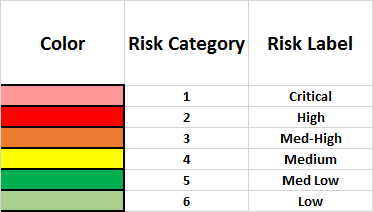
\includegraphics[width=\linewidth]{riskcats}
    \caption{Risk Categories Used in Threat Modeling}
    \label{fig:riskcats}
\end{marginfigure}


\subsection{Risk Definitions}

